
    \begin{figure}[htp]
    \centering
    \begin{subfigure}{.45\textwidth}
                \centering
                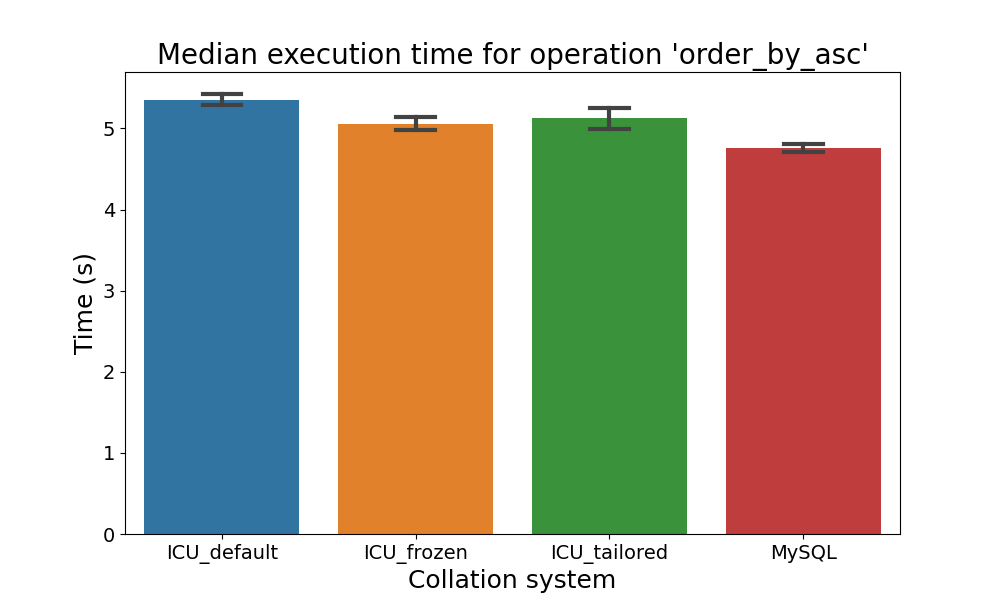
\includegraphics[width=\textwidth]{img/experiment1/en_US_utf8mb4_icu_en_US_ai_ci_vs_utf8mb4_0900_ai_ci_order_by_asc.png}
                \label{fig:experiment1_order_by_asc_en_US_utf8mb4_icu_en_US_ai_ci_vs_utf8mb4_0900_ai_ci_order_by_asc}
                \caption{English (en\_US)}
            \end{subfigure}
    \hfill
    \begin{subfigure}{.45\textwidth}
                \centering
                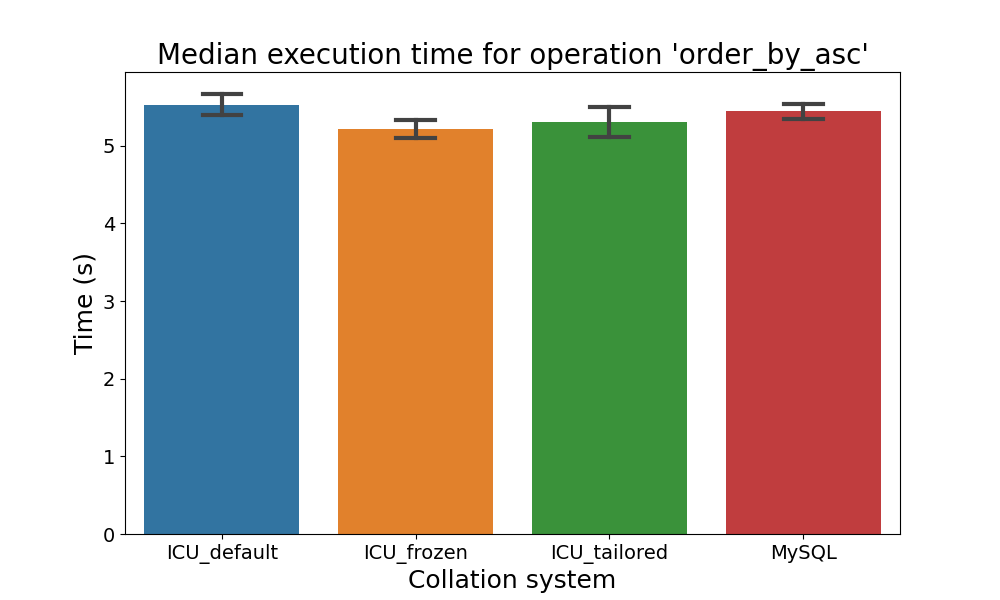
\includegraphics[width=\textwidth]{img/experiment1/nb_NO_utf8mb4_icu_nb_NO_ai_ci_vs_utf8mb4_nb_0900_ai_ci_order_by_asc.png}
                \label{fig:experiment1_order_by_asc_nb_NO_utf8mb4_icu_nb_NO_ai_ci_vs_utf8mb4_nb_0900_ai_ci_order_by_asc}
                \caption{Norwegian Bokmål (nb\_NO)}
            \end{subfigure}
    \par
    \begin{subfigure}{.45\textwidth}
                \centering
                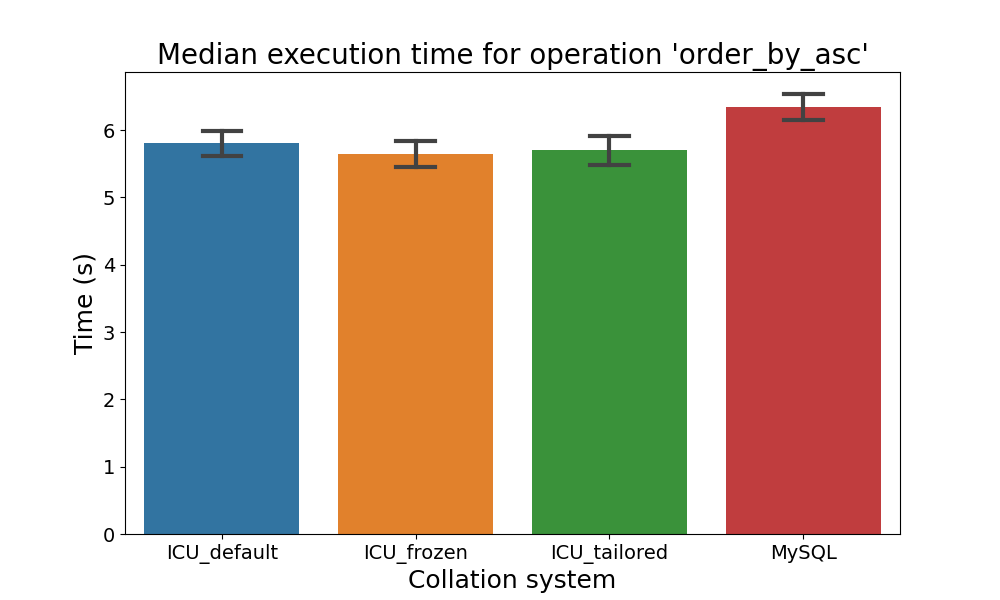
\includegraphics[width=\textwidth]{img/experiment1/zh_Hans_utf8mb4_icu_zh_Hans_as_cs_vs_utf8mb4_zh_0900_as_cs_order_by_asc.png}
                \label{fig:experiment1_order_by_asc_zh_Hans_utf8mb4_icu_zh_Hans_as_cs_vs_utf8mb4_zh_0900_as_cs_order_by_asc}
                \caption{Simplified Chinese (zh\_Hans)}
            \end{subfigure}
    \hfill
    \begin{subfigure}{.45\textwidth}
                \centering
                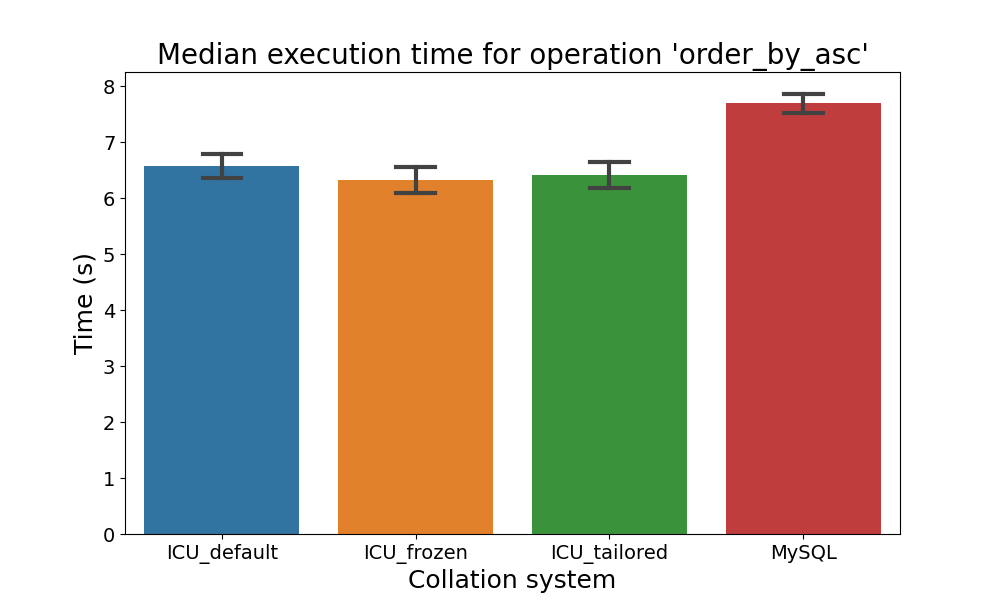
\includegraphics[width=\textwidth]{img/experiment1/ja_JP_utf8mb4_icu_ja_JP_as_cs_ks_vs_utf8mb4_ja_0900_as_cs_ks_order_by_asc.png}
                \label{fig:experiment1_order_by_asc_ja_JP_utf8mb4_icu_ja_JP_as_cs_ks_vs_utf8mb4_ja_0900_as_cs_ks_order_by_asc}
                \caption{Japanese (ja\_JP)}
            \end{subfigure}
    \caption{Comparing execution time for the ORDER BY ASC operation across various collations. Lower execution time is better. Error bars show standard deviation. These collations are all accent-, case- and (where applicable) kana-insensitive}
    \label{fig:experiment1_order_by_asc}
    \end{figure}
    